\section{Background}
In this section, we explain the infrastructure, necessary to manage base
and view tables. We start with a general description of the KV-store and 
its data model. Further, we explain the View Maintenance System that 
creates and updates the materialized views (stored in KV-store). 

\subsection{KV store}

Some KV-stores are based on a master-slave architecture, i.e. HBase;
other KV-stores run without a master, i.e. Cassandra (a leader 
is elected to perform tasks controlling the KV-store). 
In both cases a \textit{node} represents the unit of scalability -- 
as arbitrary instances can be spawned in the network (see 
Figure~\ref{fig:kv_model}). The node persists the actual data.  But in
contrast to a traditional SQL-database, a node manages only part of the 
overall data (and request load). As load grows in the KV-store, more 
nodes can be added to the system; likewise, nodes can be removed as load 
declines. The KV-store will automatically adapt to the new situation and 
integrate, respectively drop the resource. KV-stores differ in how they 
accommodate;  they also differ in how they perform load balancing and 
recovery (in face of node crashes). However, with regard to nodes, we can 
describe a set of universal events that occur in every KV-store 
(cf. Table~\ref{tab:kvs_a_events}).

A \textit{table} in a KV-store does not follow a fixed schema. It stores 
a set of table records called \textit{rows}. A row is uniquely identified by a
\textit{row key}. A row holds a variable number of \textit{columns}
(i.e., a set of column-value pairs). Columns can be further
grouped into \textit{column families}. Column families provide fast
sequential access to a subset of columns. They are determined when a
table is created and affect the way the KV-store organizes its table
files.\\ 
\textit{Key ranges} serve to partition a table into multiple
parts that can be distribute over multiple nodes.  Key ranges are
defined as an interval with a start and an end row key.  PNUTS refers
to this partitioning mechanisms as tablets, while HBase
refers to key ranges as regions. Multiple regions can be
assigned to a node, often referred to as a region server. 
In general, a KV-store can split and move key ranges between nodes to 
balance system load or to achieve a uniform distribution of data. With
regard to key ranges, we can also describe a set of universal events 
(cf. Table~\ref{tab:kvs_a_events}).


The data model of a KV-store differs from that of a
relational DBMS.  We describe a model that is representative for
today's KV-stores. The model serves throughout the paper to help
specify views and view update programs. Typically, KV-stores do not
required fixed data schemas, but rather accommodate dynamic schema
changes.

Thus, we formalize the data model of a KV-store as a map of key-value 
pairs $\{\langle k_1, v_1\rangle,..,\langle k_n,v_n\rangle\}$ described 
by a function $f:K \rightarrow V$. Systems like BigTable, HBase and 
Cassandra established data models that are multi-dimensional maps 
storing a row together with a variable number of columns per row. For 
example, the 2-dimensional case creates a structure 
$\{\langle(k_1,c_1),v_{1,1}\rangle,\langle (k_n,c_n) ,v_{n,n}\rangle\}$ 
with a composite key $(k_n,c_n)$ that maps to a value $v_{n,n}$ 
described by $f:(K,C)\rightarrow V$. In the 3-dimensional case, another 
parameter, a timestamp, for example, is added to the key, which may 
serve versioning purposes. For the intentions in this paper, the 
2-dimensional model suffices.\footnote{Our approach also works with the 
1-dimensional case, which is representative for simple key-blob stores. 
We use the 2-dimensional case here, as it is more expressive.} 


We denote a table by $A = (K, F)$, where $K$ represents the row key and 
$F$ a \textit{column family}. Column families are defined when a table 
is created. They are used in practice to group and access sets of 
column-value pairs. In terms of our data model, column families are 
optional. They can be dynamically assigned as the row is created. Let a 
base table row $a \in A$ be defined as $a=(k,\{\langle 
c_1,v_1\rangle..\langle c_n,v_n\rangle\})$. In this notation, the row 
key $k$ comes first, followed by a set of column-value pairs $\{\langle 
c_1,v_1\rangle..\langle c_n,v_n\rangle\}$ belonging to 
the column family; this more closely resembles a database row and is 
used throughout the remainder of this paper. When using multiple column 
families, we define the table as $A = (K, F_1,...F_n)$. Then the 
assignment of a column-value set to a column family $F_x$ is denoted by 
$\{..\}_x$. The corresponding row would be defined as $a=(k, \{\langle 
c_1,v_1\rangle..\langle c_i, v_i\rangle\}_1..., \{\langle 
c_{i+1},v_{i+1}\rangle.. \langle c_n,v_n\rangle\}_n)$. 

\begin{figure}[h!] 
	\centering 
	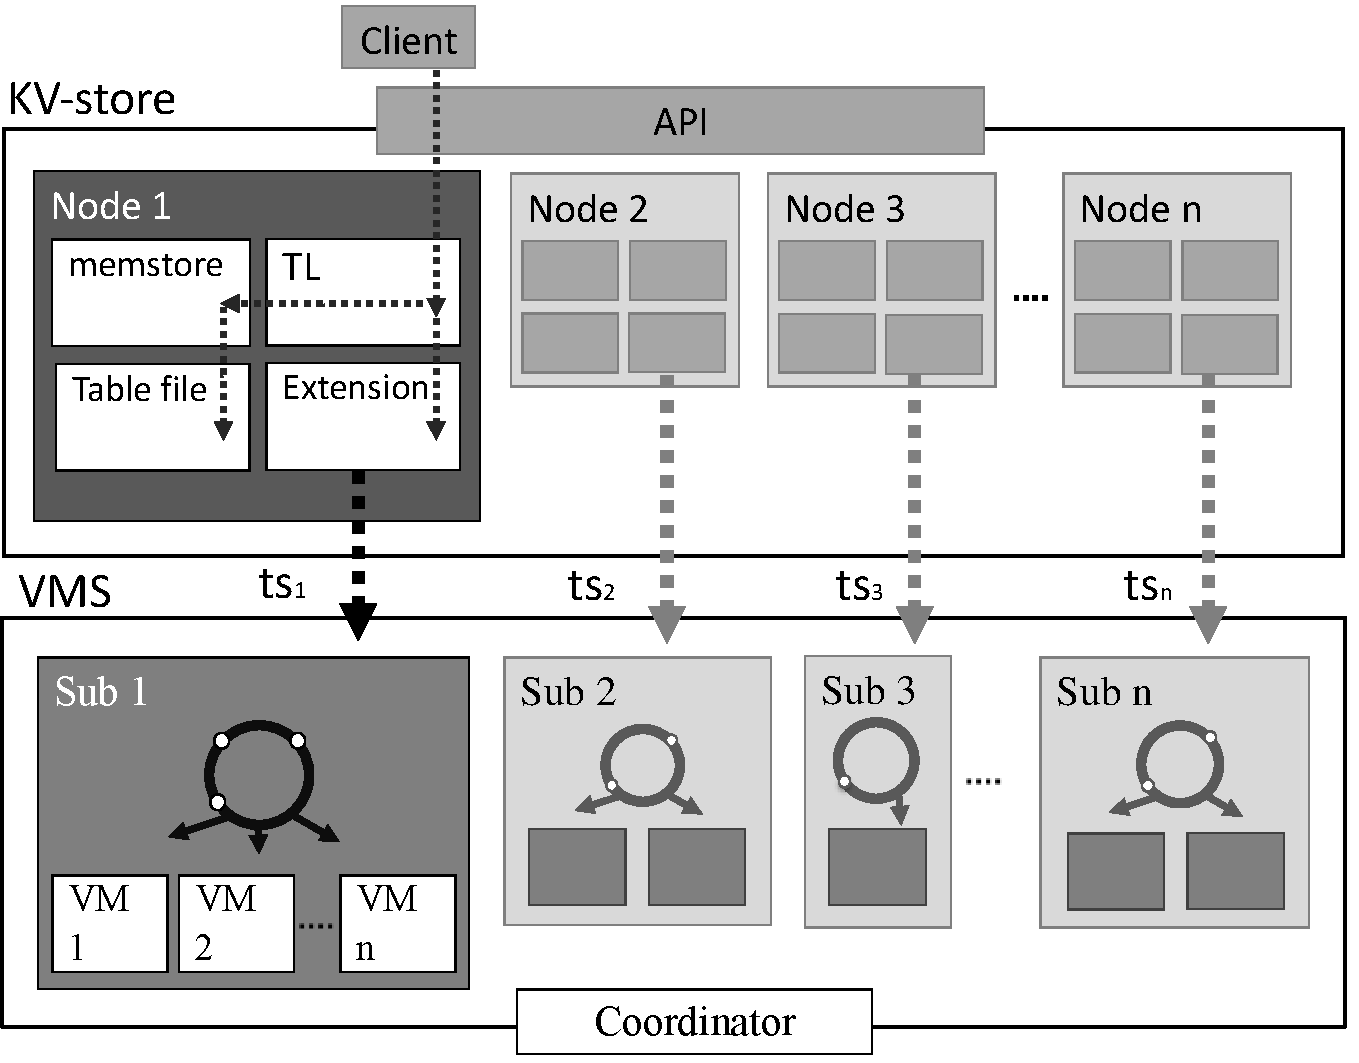
\includegraphics[width=\linewidth]{figures/SystemOverview}  
	\caption{System Overview} 
	\label{fig:system_overview} 
\end{figure} 



The KV-store writes operations, that is client requests, to the TL,
but not entire table rows.  In contrast, a table row stores the row
state, which may result from multiple client requests.  Then, an 
operation $t \in T$ can easily be defined over table row $a \in A$,
with $T = type(A)$  and $type \in \{put, delete\}$. A put operation in
the transaction log is denoted as $t=put (k, \{\langle c_1,v_1\rangle..\langle
c_n,v_n\rangle\})$. A put inserts or updates the column values at the
specified row key. A delete operation $t \in T$ is defined as
$t=delete (k, \{\langle c_1,\emptyset\rangle..\langle
c_n,\emptyset\rangle\})$.  Note that we are leaving the values 
empty; the client just specifies the row key and columns that are to
be deleted. A stream -- respectively, the output of one node's transaction log --
is denoted as a sequence of operations $ts \in TS=(T_1,..,T_n)$. Finally, we can
define the complete output of the KV-store as a set of operation 
streams as $ts_1,..ts_n \in TS$. 

\subsection{View Maintenance System}

%The streams consist of insert and put operation $t_p$ and a delete 
%operation $t_d$ into the base table. These 
%two operation types are the only way a client can modify the base table 
%and, hence, affect the view table. We denote the two operation types, 
%as they are written to the TL, in the general form $t_p=put(A(k,\{\langle 
%c_1, v_1\rangle, \langle c_2,v_2\rangle\}))$ and $t_d=delete( A(k))$. 

The View Maintenance System receives updates from the KV-store in form
of operation streams (see Figure~\ref{fig:system_overview}). Every node
of the KV-store produces a local transaction stream ($ts_1,..,ts_n$);every 
stream of operations is handled by a subsystem of the VMS. The subsystem 
parallizes view update computation: it distributes the updates to a
scalable number of view managers. A view manager actually applies the
update operation to the view table. First, it looks up the view tables 
 defined over the base, then it retrieves the corresponding view record, 
adds the delta to it, and writes back the result to the view.

We express view tables in the VMS with the help of relational algebra 
(e.g., we define a \texttt{SELECTION} as $S=\sigma_{c_1 < x}(A)$ over a 
base table $A$). Defining a view table over a base table is equivalent
to connection the output stream of base table operations with the input
stream of view table input operations. The VMS is also capable of 
defining view tables over view tables (e.g. we define a \texttt{PROJECTION}
view as $P=\pi_{c_1,c_2}(S)$). Thus,
we can concatenate multiple different view types; the VMS will update the
view chain subsequently. It will receive the base table update, apply the
update to the \texttt{SELECTION} view, and apply the result of the first
update to the \texttt{PROJECTION} view.